%==============================================================================
\documentclass[MathematicsNumericsDerivationsAndOpenFOAM.tex]{subfiles}
\begin{document}
%==============================================================================


\section{守恒动量方程}
\label{SECTION::momentum}
%
%
下面将讨论动量方程的推导,它也被称为纳维-斯托克斯方程。
	
守恒动量方程的推导与连续性方程相似。同样,我们将使用体积元素d$V$。与质量守恒方程相比,动量方程的主要区别如下。动量的数量是一个矢量,而不是一个标量。因此,动量不仅是通过体积元素表面的通量来传输/对流的。

%
%
	一般来说,我们可以在体积d$V$内定义动量传输及其变化如下。
%
%
\begin{equation}
\left[
 \vphantom{\begin{matrix} . \\ . \\ . \\ . \end{matrix}}
 \begin{matrix}
  \rmm{rate~of}\\
  \rmm{momentum}\\
  \rmm{accumulation}
 \end{matrix}
\right]
=
\left[
 \begin{matrix}
  \rmm{rate~of}\\
  \rmm{momentum}\\
  \rmm{entering~the}\\
  \rmm{volume}
 \end{matrix}
\right]
-
\left[
 \begin{matrix}
  \rmm{rate~of}\\
  \rmm{momentum}\\
  \rmm{leaving~the}\\
  \rmm{volume}
 \end{matrix}
\right]
+
\left[
 \vphantom{\begin{matrix} . \\ . \\ . \\ . \end{matrix}}
 \begin{matrix}
  \rmm{sum~of~forces}\\
  \rmm{that~act~on}\\
  \rmm{the~volume}
 \end{matrix}
\right] .
\label{EQUATION::momentum}
\end{equation}
%
%
	图 \ref{Abb_Grundlagen_2_Impulserhaltung}显示了与图 \ref{figure::massFigure}中给出的相同的体积元素,但现在包括了另一种作用于表面的传输现象(只介绍了$x$方向)。这种动量的传输是基于分子效应的。分子传输总是作用于表面的法线和切线,是矢量的结果或属性。
%
%
%
%
\begin{figure}[!b]
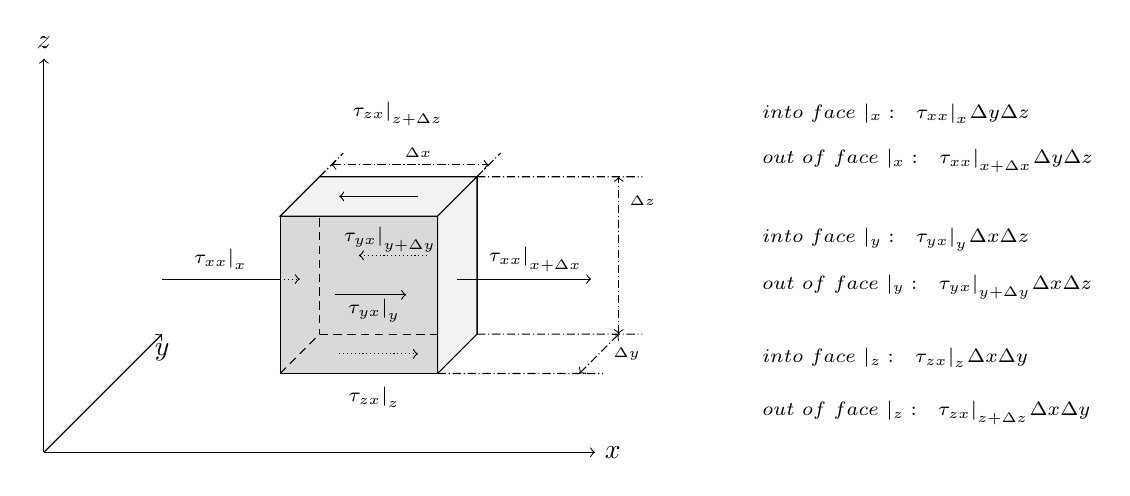
\begin{tikzpicture}
% Koordinatensystem
\draw[->] (0,0) -- (7,0) node[right] {$x$} coordinate(x axis);
\draw[->] (0,0) -- (0,5) node[above] {$z$} coordinate(y axis);
\draw[->] (0,0) -- (1.5,1.5) node[below] {$y$} coordinate(z axis);

% Quader
\draw [fill=gray!30] (3,1) -- (5,1) -- (5,3) -- (3,3) -- (3,1) ;

\draw [densely dashed] (3.5,1.5) -- (5.5,1.5);
\draw [] (5.5,1.5) -- (5.5,3.5) -- (3.5,3.5);
\draw [densely dashed] (3.5,3.5) -- (3.5,1.5);

\draw  [densely dashed] (3,1) -- (3.5,1.5);
\draw  [fill=gray!10] (5,1) -- (5.5,1.5) -- (5.5,3.5) -- (5,3) -- (5,1);
\draw  [fill=gray!10] (5,3) -- (5.5,3.5) --  (3.5,3.5) -- (3,3) -- (5,3);

%\draw (3,1) -- (3.5,3.5);
%\draw (3,3) -- (3.5,1.5);

% Pfeile
% rechts nach links
\draw [densely dotted, ->] (3,2.2) -- (3.25,2.2);


\draw [] (1.5,2.2) -- (3,2.2);

\draw [->] (5.25,2.2) -- (6.95,2.2);


% unten und oben
\draw [densely dotted, ->] (3.75,1.25) -- (4.75,1.25);
%\draw [-] (4.25,0.25) -- (4.25,1);
\draw [->] (4.75,3.25) -- (3.75,3.25);

% vorn und hinten
\draw [->] (3.7,2) -- (4.6,2);
\draw [densely dotted, <-] (4.0,2.5) -- (4.9,2.5);


% Punkte für Gleichungen
\node at (2.25,2.45) {\scriptsize $\tau_{xx}|_{_x}$};
\node at (6.25,2.45) {\scriptsize $\tau_{xx}|_{_{x+\Delta x}}$};

\node at (4.2,0.7) {\scriptsize $\tau_{zx}|_{_z}$};
\node at (4.5,4.3) {\scriptsize $\tau_{zx}|_{_{z+\Delta z}}$};

\node at (4.4,2.7) {\scriptsize $\tau_{yx}|_{_{y+\Delta y}}$};
\node at (4.2,1.8) {\scriptsize $\tau_{yx}|_{_y}$};



% Linien für dx dy dz
\draw [densely dashdotted] (5,1) -- (7.1,1)
	 (5.5,1.5) -- (7.6,1.5)
	 (5.5,3.5) -- (7.6, 3.5)
	 (3.5,3.5) -- (3.8,3.8)
	 (5.5,3.5) -- (5.8,3.8);

\draw [<->,densely dashdotted] (6.8,1) -- (7.3,1.5);
\node at (7.4,1.25) {\tiny $\Delta y$};

\draw [<->,densely dashdotted] (7.3,1.5) -- (7.3,3.5);
\node at (7.6,3.2) {\tiny $\Delta z$};

\draw [<->,densely dashdotted] (3.65,3.65) -- (5.65,3.65);
\node at (4.75,3.8) {\tiny $\Delta x$};

% Volumenpunkt
%\node at (4.25,2.25) {\tiny $\bullet$};
%\node at (4.5,2.25) {\tiny d$V$};



\node at (9,4.3) 	[right] {\scriptsize $\rmm{into~face~}|_x:~ ~ \tau_{xx}|_{_x} \Delta y \Delta z$};
\node at (9.0,3.7) 	[right] {\scriptsize $\rmm{out~of~face~}|_x:~ ~ \tau_{xx}|_{_{x + \Delta x}} \Delta y \Delta z$};

\node at (9,2.7) 	[right] {\scriptsize $\rmm{into~face~}|_y:~ ~ \tau_{yx}|_{_y} \Delta x \Delta z$};
\node at (9,2.1) 	[right] {\scriptsize $\rmm{out~of~face~}|_y:~ ~ \tau_{yx}|_{_{y + \Delta y}} \Delta x \Delta z$};

\node at (9,1.2) 	[right] {\scriptsize $\rmm{into~face~}|_z:~ ~ \tau_{zx}|_{_z} \Delta x \Delta y$};
\node at (9,0.5) 	[right] {\scriptsize $\rmm{out~of~face~}|_z:~ ~ \tau_{zx}|_{_{z + \Delta z}} \Delta x \Delta y$};
%
%
%
%
\end{tikzpicture}
\caption{Molecular transport of the momentum in $x$-direction in an arbitrary small volume element d$V$.}
\label{Abb_Grundlagen_2_Impulserhaltung}
\end{figure}
%
%
其他改变体积内动量的现象是以力的总和给出的。例如,我们可以有重力加速度和作用在体积上的压力。

在图 \ref{Abb_Grundlagen_2_Impulserhaltung}的右边,给出了通过分子传输效应将动量的$x$分量通过表面传输的条款。
 
%
%
\subsubsection{在$x$方向的动量传输}
%
%
%
 动量的$x$分量通过对流进入体积元素,通过所有六个面进行传输。因此,动量的对流可以与质量的对流传输类似地得到。然而,现在我们必须照顾到 \textbf{vector}量。因此,$x$方向的动量在面$|_{_x}$处进入体积,通过面$|_{_{x+\Delta x}}$离开体积;与连续性方程相同。然而,也有可能动量的$x$分量通过面的$y$和$z$方向传输(分子传输)。因此,我们可以写出对流引起的动量传输;它只是$x$方向的速度乘以通过我们所看的面的\textbf{flux}(牛顿第二定律)。
%
%
\begin{align*}
 \rmm{into~face~}&|_{_x}: ~~~~~~~
 (\rho u_x)u_x|_{_x} ~, \\
 \rmm{out~of~face~}&|_{_{x+\Delta x}}: ~~~
 (\rho u_x)u_x |_{_{x+\Delta x}} ~,
 \\
 \rmm{into~face~}&|_{_y} : ~~~~~~~
 (\rho u_y)u_x |_{_y} ~, \\
 \rmm{out~of~face~}&|_{_{y+\Delta y}} : ~~~
 (\rho u_y)u_x |_{_{y+\Delta y}} ~,
 \\
 \rmm{into~face~}&|_{_z} : ~~~~~~~
 (\rho u_z)u_x |_{_z} ~, \\
 \rmm{out~of~face~}&|_{_{z+\Delta z}} : ~~~
 (\rho u_z)u_x |_{_{z+\Delta z}} ~.
\end{align*}
%
%
	在结合这些术语并使用面域后,我们得到:
%
%
\begin{align*}
  &\left(
    (\rho u_x)u_x |_{_x} - (\rho u_x)u_x |_{_{x+\Delta x}}
  \right)
  \Delta y \Delta z \\
  +&\left(
    (\rho u_y)u_x |_{_y} - (\rho u_y)u_x |_{_{y+\Delta y}}
  \right)
  \Delta x \Delta z  \\
  +&\left(
    (\rho u_z)u_x |_{_z} - (\rho u_z)u_x |_{_{z+\Delta z}}
  \right)
  \Delta x \Delta y ~.
\end{align*}
%
%
%
%
\subsubsection{分子在$x$方向的动量传输}
%
%
%
%
	此外,如图\ref{Abb_Grundlagen_2_Impulserhaltung}所示,由于分子效应,动量的$x$分量被输送。这种效应是基于速度差(速度梯度)。正如我们在图\ref{Abb_Grundlagen_2_Impulserhaltung}中看到的那样,出现了不同的项,包括法向分量$\tau_{xx}$或切向分量$\tau_{yx}$或$\tau_{zx}$。因此,通过表面的$x$动量的分子传输可以写成。
%
%
\begin{align*}
  &\left(
    \tau_{xx} |_{_x} - \tau_{xx} |_{_{x+\Delta x}}
  \right)
  \Delta y \Delta z \\
  +&\left(
    \tau_{yx} |_{_y} - \tau_{yx} |_{_{y+\Delta y}}
  \right)
  \Delta x \Delta z \\
  +&\left(
    \tau_{zx} |_{_z} - \tau_{zx} |_{_{z+\Delta z}}
  \right)
  \Delta x \Delta y ~.
\end{align*}
%
%
这些通量视为应力。$\tau_{xx}$表示垂直于我们所看的方向的应力(这里是 $\rmm{face}~|_{_x}$和$\rmm{face}~|_{_{x+\Delta x}}$),$\tau_{yx}$、$\tau_{zx}$表示$x$方向的切向应力,相对于指数作用在面上。所有这些应力都被称为剪切应力,因为它们是关于引入剪切的速度梯度而产生的。
%
%
%
%
\subsubsection{影响动量的其他力}
%
%
%
      在大多数科学和工程任务中,影响动量的最基本力量是压力和重力。压强作用于体积元素的表面,而引力则直接作用于体积。因此,我们可以根据压力和引力推导出$x$动量的变化,如下所示。
%
%
\begin{equation*}
  \left(
    p|_{_x} - p|_{_{x+\Delta x}}
  \right)
  \Delta y \Delta z
+
  \rho g_x \Delta x \Delta y \Delta z ~.
\end{equation*}
%
%
%
%
\subsubsection{守恒动量方程}
%
%
      在我们有了所有的条款之后------忽略其他的影响因素,如表面张力等等------,方程(\ref{EQUATION::momentum})可以用上面得出的相应的数学表达式来重构。当然,任意体积元素内部的动量积累由以下公式给出。
%
%
$$
 \frac{\Delta}{\Delta t} \rho u_x \Delta x \Delta y \Delta z ~.
$$
%
%
      因此,对于$x$方向的动量,我们可以写出
%
%
\begin{align*}
  \frac{\Delta}{\Delta t} \rho u_x \Delta x \Delta y \Delta z
=
  &\left(
  (\rho u_x)u_x|_{_x} - (\rho u_x)u_x|_{_{x+\Delta x}}
  \right) \Delta y \Delta z
 \\
  +&\left(
  (\rho u_y)u_x|_{_y} - (\rho u_y)u_x|_{_{y+\Delta y}}
  \right) \Delta x \Delta z
 \\
 +&\left(
  (\rho u_z)u_x|_{_z} - (\rho u_z)u_x|_{_{z+\Delta z}}
  \right) \Delta x \Delta y
 \\
 +&\left(
  \tau_{xx}|_{_x} - \tau_{xx}|_{_{x+\Delta x}}
  \right)\Delta y \Delta z
 \\
  +&\left(
  \tau_{yx}|_{_y} - \tau_{yx}|_{_{y+\Delta y}}
  \right) \Delta x \Delta z
 \\
  +&\left(
  \tau_{zx}|_{_z} - \tau_{zx}|_{_{z+\Delta z}}
  \right) \Delta x \Delta y
 \\
  +&\left(
  p|_{_x} - p|_{_{x+\Delta x}}
  \right) \Delta y \Delta z
 \\
  +&\rho g_x  \Delta x \Delta y \Delta z ~.
  \numberthis
\end{align*}
%
%
现在,通过将整个方程除以体积d$V$,可以看出。
%
%
\begin{align*}
   \frac{\Delta}{\Delta t} \rho u_x
&=
  \frac{(\rho u_x)u_x|_{_x} - (\rho u_x)u_x|_{_{x+\Delta x}}}{\Delta x}
+
  \frac{(\rho u_y)u_x|_{_y} - (\rho u_y)u_x|_{_{y+\Delta y}}}{\Delta y}
 \\
&+
  \frac{(\rho u_z)u_x|_{_z} - (\rho u_z)u_x|_{_{z+\Delta z}}}{\Delta z}
+
  \frac{\tau_{xx}|_{_x} - \tau_{xx}|_{_{x+\Delta x}}}{\Delta x}
+
  \frac{\tau_{yx}|_{_y} - \tau_{yx}|_{_{y+\Delta y}}}{\Delta y}
 \\
&+
  \frac{\tau_{zx}|_{_z} - \tau_{zx}|_{_{z+\Delta z}}}{\Delta z}
+
  \frac{p|_{_x} - p|_{_{x+\Delta x}}}{\Delta x}
+
  \rho g_x ~.
  \numberthis
\end{align*}
%
%
	最后,我们利用无限小的体积元素(\ref{EQUATION::infty})和时间范围(\ref{EQUATION::inftyTime})的假设来重写动量方程的$x$分量。然后,动量的$x$分量被写成:
%
%
\begin{equation}\boxed{\begin{aligned}
  \frac{\partial}{\partial t} \rho u_x
=
 &-\left(
      \frac{\partial}{\partial x} \rho u_x u_x
      +\frac{\partial}{\partial y} \rho u_y u_x
      +\frac{\partial}{\partial z} \rho u_z u_x
  \right)\\
 &-\left(
      \frac{\partial}{\partial x}  \tau_{xx}
      +\frac{\partial}{\partial y}  \tau_{yx}
      +\frac{\partial}{\partial z}  \tau_{zx}
  \right)
  -
  \frac{\partial p}{\partial x}
  +
  \rho g_x
  \label{EQUATION::momentumX}
\end{aligned}} ~.\end{equation}
%
%
    其他两个空间分量的推导与$x$分量相同。因此,只给出最后的表述。对于动量的$y$分量,我们得到
%
%
\begin{equation}\boxed{\begin{aligned}
  \frac{\partial}{\partial t} \rho u_y
=
 &-\left(
      \frac{\partial}{\partial x} \rho u_x u_y
      +\frac{\partial}{\partial y} \rho u_y u_y
      +\frac{\partial}{\partial z} \rho u_z u_y
  \right)\\
 &-\left(
      \frac{\partial}{\partial x}  \tau_{xy}
      +\frac{\partial}{\partial y}  \tau_{yy}
      +\frac{\partial}{\partial z}  \tau_{zy}
  \right)
  -
  \frac{\partial p}{\partial y}
  +
  \rho g_y
  \label{EQUATION::momentumY}
\end{aligned}}~,
\end{equation}
%
%
	而对于$z$分量,我们实现了
%
%

\begin{equation}
\boxed{
\begin{aligned}
  \frac{\partial}{\partial t} \rho u_z
=
 &-\left(
      \frac{\partial}{\partial x} \rho u_x u_z
      +\frac{\partial}{\partial y} \rho u_y u_z
      +\frac{\partial}{\partial z} \rho u_z u_z
  \right)\\
 &-\left(
      \frac{\partial}{\partial x}  \tau_{xz}
      +\frac{\partial}{\partial y}  \tau_{yz}
      +\frac{\partial}{\partial z}  \tau_{zz}
  \right)
  -
  \frac{\partial p}{\partial z}
  +
  \rho g_z
  \label{EQUATION::momentumZ}
\end{aligned}
}~.
\end{equation}
%
%
	引入重力加速度矢量\textbf{g},压力梯度$\nabla p$和剪切率张量$\boldsymbol \tau$,定义为:
%
%
\begin{equation*}
    \nabla p
=
\left(
  \begin{matrix}
    \frac{\partial p}{\partial x} \\
    \frac{\partial p}{\partial y} \\
    \frac{\partial p}{\partial z} \\
  \end{matrix}
  \right),
  ~ ~ ~ ~ ~ ~ ~
\boldsymbol \tau
=
\left[
 \begin{matrix}
  \tau_{xx} ~~~~ \tau_{xy} ~~~~ \tau_{xz} \\
  \tau_{yx} ~~~~ \tau_{yy} ~~~~ \tau_{yz} \\
  \tau_{zx} ~~~~ \tau_{zy} ~~~~ \tau_{zz}
 \end{matrix}
\right],
  ~ ~ ~ ~ ~ ~ ~
\textbf{g}
=
\left(
 \begin{matrix}
  g_x \\
  g_y \\
  g_z
 \end{matrix}
\right),
\end{equation*}
%
%
	我们可以用矢量形式写出守恒动量方程:
%
%
\begin{equation}
 \boxed{
    \frac{\partial}{\partial t} \rho \textbf{U}
=
    -   \nabla \bullet \left(\rho\textbf{U} \otimes \textbf{U}\right)
    -   \nabla \bullet \boldsymbol \tau
    -   \nabla p
    + \rho\textbf{g}
 }~.
 \label{EQUATION::momentumDiv}
\end{equation}
%
%
    \textbf{备注},   如果我们在后面介绍剪切率张量的定义$\boldsymbol \tau$,那么剪切率张量的负号就会改变。
%
%
%
%
%
\subsection{推导过程}
%
%
    下面将研究证明方程(\ref{EQUATION::momentumDiv})的结果是(\ref{EQUATION::momentumX})、(\ref{EQUATION::momentumY})和(\ref{EQUATION::momentumZ})。
%
%
    为了更加清楚说明,我们将分别关注每一个项。从第一项开始,即时间导数,我们得到
%
%
\begin{equation}
  \frac{\partial}{\partial t} \rho \textbf{U}
=
  \left(
  \begin{matrix}
      \frac{\partial}{\partial t} \rho u_x \\
      \frac{\partial}{\partial t} \rho u_y \\
      \frac{\partial}{\partial t} \rho u_z
  \end{matrix}
  \right)
\overset{!}{=}
\begin{cases}
  \frac{\partial}{\partial t} \rho u_x  ~~~ \rmm{of~}x-\rmm{momentum}\\
  \frac{\partial}{\partial t} \rho u_y  ~~~ \rmm{of~}y-\rmm{momentum}\\
  \frac{\partial}{\partial t} \rho u_z  ~~~ \rmm{of~}z-\rmm{momentum}
\end{cases} ~.
\end{equation}
%
%
    正如我们所看到的,时间导数项的结果与我们在笛卡尔公式中的三个项相同。第二个项包含了由通量$\rho\textbf{U}$引起的对流所带来的动量传输。为了评估这个项,我们需要数学(\ref{EQUATION::dyadic})和(\ref{EQUATION::divTensor})。
%
%
\begin{equation*}
 -   \nabla \bullet \left(\rho\textbf{U} \otimes \textbf{U}\right)
=
-   \nabla \bullet
  \left\{
  \rho
  \left(
  \begin{matrix}
    u_x \\
    u_y \\
    u_z
  \end{matrix}
  \right)
\otimes
\left(
  \begin{matrix}
    u_x \\
    u_y \\
    u_z
  \end{matrix}
  \right)
  \right\}
=
-   \nabla \bullet
  \left\{
  \rho
  \left[
  \begin{matrix}
    u_x u_x ~~~~ u_x u_y ~~~~ u_x u_z \\
    u_y u_x ~~~~ u_y u_y ~~~~ u_y u_z \\
    u_z u_x ~~~~ u_z u_y ~~~~ u_z u_z
  \end{matrix}
  \right]
  \right\}
\end{equation*}
%
%
%
\begin{equation*}
= -   \nabla \bullet
  \left[
  \begin{matrix}
    \rho u_x u_x ~~~~ \rho u_x u_y ~~~~ \rho u_x u_z \\
    \rho u_y u_x ~~~~ \rho u_y u_y ~~~~ \rho u_y u_z \\
    \rho u_z u_x ~~~~ \rho u_z u_y ~~~~ \rho u_z u_z
  \end{matrix}
  \right]
=
- \left(
  \begin{matrix}
    \frac{\partial}{\partial x} \\
    \frac{\partial}{\partial y} \\
    \frac{\partial}{\partial z}
  \end{matrix}
  \right)
  \bullet
  \left[
  \begin{matrix}
    \rho u_x u_x ~~~~ \rho u_x u_y ~~~~ \rho u_x u_z \\
    \rho u_y u_x ~~~~ \rho u_y u_y ~~~~ \rho u_y u_z \\
    \rho u_z u_x ~~~~ \rho u_z u_y ~~~~ \rho u_z u_z
  \end{matrix}
  \right]
\end{equation*}
%
%
\begin{equation*}
= - \left[
  \begin{matrix}
    \frac{\partial}{\partial x} \rho u_x u_x +
    \frac{\partial}{\partial y} \rho u_y u_x +
    \frac{\partial}{\partial z} \rho u_z u_x \\
    \frac{\partial}{\partial x} \rho u_x u_y +
    \frac{\partial}{\partial y} \rho u_y u_y +
    \frac{\partial}{\partial z} \rho u_z u_y \\
    \frac{\partial}{\partial x} \rho u_x u_z +
    \frac{\partial}{\partial y} \rho u_y u_z +
    \frac{\partial}{\partial z} \rho u_z u_z
  \end{matrix}
  \right]
\overset{!}{=}
\begin{cases}
  -\left(
      \frac{\partial}{\partial x} \rho u_x u_x
      +\frac{\partial}{\partial y} \rho u_y u_x
      +\frac{\partial}{\partial z} \rho u_z u_x
  \right)% ~~~ \rmm{of~}x- \rmm{mom.}\\
  \\
  -\left(
      \frac{\partial}{\partial x} \rho u_x u_y
      +\frac{\partial}{\partial y} \rho u_y u_y
      +\frac{\partial}{\partial z} \rho u_z u_y
  \right)% ~~~ \rmm{of~}y- \rmm{mom.}\\
  \\
  -\left(
      \frac{\partial}{\partial x} \rho u_x u_z
      +\frac{\partial}{\partial y} \rho u_y u_z
      +\frac{\partial}{\partial z} \rho u_z u_z
  \right)% ~~~ \rmm{of~}z- \rmm{mom.}
\end{cases}
  .
\end{equation*}
%
%
    同样,我们可以看到,这些项是相等的,我们最终得到了相同的方程组。现在我们研究第三个项,它描述了由于速度梯度而产生的剪切。 使用剪切率张量$\boldsymbol \tau$的惯例(\ref{EQUATION::divTensor}),我们得到。
%
%
\begin{equation*}
  -  \nabla \bullet \boldsymbol \tau
=
  -  \nabla \bullet
  \left[
  \begin{matrix}
  \tau_{xx} ~~~~ \tau_{xy} ~~~~ \tau_{xz} \\
  \tau_{yx} ~~~~ \tau_{yy} ~~~~ \tau_{yz} \\
  \tau_{zx} ~~~~ \tau_{zy} ~~~~ \tau_{zz}
  \end{matrix}
  \right]
=
\end{equation*}
\begin{equation*}
- \left[
  \begin{matrix}
  \frac{\partial}{\partial x}\tau_{xx} + \frac{\partial}{\partial y} \tau_{yx} + \frac{\partial}{\partial z} \tau_{zx} \\
  \frac{\partial}{\partial x}\tau_{xy} + \frac{\partial}{\partial y} \tau_{yy} + \frac{\partial}{\partial z}\tau_{zy} \\
  \frac{\partial}{\partial x}\tau_{xz} + \frac{\partial}{\partial y} \tau_{yz} + \frac{\partial}{\partial z} \tau_{zz}
  \end{matrix}
  \right]
\overset{!}{=}
  \begin{cases}
  -\left(
      \frac{\partial}{\partial x}  \tau_{xx}
      +\frac{\partial}{\partial y}  \tau_{yx}
      +\frac{\partial}{\partial z}  \tau_{zx}
  \right) ~ \rmm{of~}x ~ \rmm{momentum} \\
  -\left(
      \frac{\partial}{\partial x}  \tau_{xy}
      +\frac{\partial}{\partial y}  \tau_{yy}
      +\frac{\partial}{\partial z}  \tau_{zy}
  \right) ~ \rmm{of~}y ~ \rmm{momentum} \\
    -\left(
      \frac{\partial}{\partial x}  \tau_{xz}
      +\frac{\partial}{\partial y}  \tau_{yz}
      +\frac{\partial}{\partial z}  \tau_{zz}
  \right) ~ \rmm{of~}z ~ \rmm{momentum}
  \end{cases}
  .
\end{equation*}
%
%
    最后对压力和重力加速度项进行了分析。对于压力项,我们需要方程(\ref{EQUATION::gradientScalar})的定义,对于重力项,我们需要方程(\ref{EQUATION::simple})。由此可见。
%
%
\begin{equation*}
  -  \nabla p
=
  -
  \left(
  \begin{matrix}
   \frac{\partial}{\partial x} \\
   \frac{\partial}{\partial y} \\
   \frac{\partial}{\partial z}
  \end{matrix}
  \right) p
=
-
  \left(
  \begin{matrix}
   \frac{\partial p}{\partial x} \\
   \frac{\partial p}{\partial y} \\
   \frac{\partial p}{\partial z}
  \end{matrix}
  \right)
\overset{!}{=}
  \begin{cases}
  -\frac{\partial p}{\partial x} ~ \rmm{of~}x ~ \rmm{momentum} \\
  -\frac{\partial p}{\partial y} ~ \rmm{of~}y ~ \rmm{momentum} \\
  -\frac{\partial p}{\partial z} ~ \rmm{of~}z ~ \rmm{momentum}
  \end{cases},
\end{equation*}
\begin{equation*}
  \rho \textbf{g}
=
  \rho
  \left(
  \begin{matrix}
    g_x \\
    g_y \\
    g_z
  \end{matrix}
  \right)
=
  \left(
  \begin{matrix}
    \rho g_x \\
    \rho g_y \\
    \rho g_z
  \end{matrix}
  \right)
\overset{!}{=}
  \begin{cases}
  \rho g_x ~ \rmm{of~}x ~ \rmm{momentum} \\
  \rho g_y ~ \rmm{of~}y ~ \rmm{momentum} \\
  \rho g_z ~ \rmm{of~}z ~ \rmm{momentum}
  \end{cases} .
\end{equation*}
%
%
正如我们现在所证明的那样,矢量形式最后变成了直角坐标形式。
	 
如果我们现在想解决这个方程,有必要知道剪切率张量$\boldsymbol \tau$。我们将在第1章中研究这个量 \ref{CHAPTER::shearrate}。动量方程的进一步表述可以在 \ref{CHAPTER::DivationsOfMomentum}一章中找到。动量方程在  \OF 中的实现将在 \ref{CHAPTER::ShearRateTensorFunctions}一章中讨论;特别是对扩散项的处理。 请记住,方程(\ref{EQUATION::momentumDiv})包括了的重力加速度和压力。 如果有更多的现象(力)影响到动量方程,这些条款必须被考虑在内。
%
%
%
\subsection{守恒动量方程的积分形式}
%
%
   动量方程的积分形式(\ref{EQUATION::momentumDiv})可以通过使用高斯定理(\ref{EQUATION::gausstheorem})获得。由此可见
%
%
%
\begin{equation}
 \boxed{
    \frac{\partial}{\partial t} \int \rho \textbf{U} \mathrm{d}V
=
    -   \oint (\rho\textbf{U} \otimes \textbf{U}) \cdot \textbf{n} \mathrm{d}S
    -   \oint \boldsymbol \tau  \cdot \textbf{n} \mathrm{d}S
    -   \oint p\textbf{I} \cdot \textbf{n} \mathrm{d}S
    + \int \rho\textbf{g}  \mathrm{d}V
 } ~.
\end{equation}
%
%
%
\subsection{非守恒动量方程}
%
%
    我们可以用连续性方程(\ref{EQUATION::massCompressible})来处理守恒动量方程。因此,我们得到了非守恒的形式。为此,我们首先考虑方程(\ref{EQUATION::momentumDiv}),并通过使用乘积规则分割时间和对流项。时间导数变成
%
%
\begin{equation}
  \frac{\partial}{\partial t} \rho \textbf{U}
=
  \rho \frac{\partial}{\partial t} \textbf{U} + \textbf{U} \frac{\partial}{\partial t} \rho ~,
\end{equation}
%
%
  和对流项可以用公式重写 (\ref{EQUATION::productRuleVV})。由此可见

%
%
\begin{equation}
  \nabla \bullet \left(\rho\textbf{U} \otimes \textbf{U}\right)
=
  \underbrace{\rho\textbf{U} \bullet \underbrace{\nabla \otimes \textbf{U}}_{\mathrm{gradient}}}_{\mathrm{inner~product}} + \textbf{U} \underbrace{\nabla \bullet (\rho\textbf{U})}_{\mathrm{divergence}} ~.
\end{equation}
%
%
    将这些条款替换到方程(\ref{EQUATION::momentumDiv})中,并将对流条款放到LHS中,我们最终得到了。
%
%
\begin{equation}
   \rho \frac{\partial}{\partial t} \textbf{U} + \textbf{U} \frac{\partial}{\partial t} \rho
+
   \rho\textbf{U} \bullet \nabla \otimes \textbf{U} + \textbf{U} \nabla \bullet (\rho\textbf{U})
=
   .~.~.
\end{equation}
%
%
    经过分析方程,我们可以看到,我们可以取出$\rho$和    $\textbf{U}$:
%
%
\begin{equation}
   \rho \left[\frac{\partial}{\partial t} \textbf{U} + \textbf{U} \bullet \nabla \otimes \textbf{U}\right]
+
\textbf{U} \underbrace{\left[\cancel{\frac{\partial}{\partial t} \rho + \nabla \bullet (\rho\textbf{U})}\right]}_{\mathrm{continuity}}
=
   .~.~.
\end{equation}
%
%
    很明显,由于连续性方程的存在,第二项是零。应用总导数的定义(\ref{EQUATION::totalDerivative}),我们可以把动量方程的非保守形式写成
%
%
\begin{equation}
  \rho \frac{\mathrm{D}\textbf{U}}{\mathrm{D}t}
=
    -   \nabla \bullet \boldsymbol \tau
    -   \nabla p
    + \rho\textbf{g}
\label{EQUATION::momentumDivNon}
\end{equation}
%
%
    \textbf{备注}: 如前所述,在我们引入剪切率分量$\tau_{ii}$的定义后,RHS上第一个项的负号将消失。
%
%
%
%
%

%==============================================================================
\end{document}
%==============================================================================
